%%%%%%%%%%%%%%%%%%%%%%%%%%%%%%%%%%%%%%%%%
% Szablon pracy dyplomowej
% Wydział Informatyki 
% Zachodniopomorski Uniwersytet Technologiczny w Szczecinie
% autor Joanna Kołodziejczyk (jkolodziejczyk@zut.edu.pl)
% Bardzo wczesnym pierwowzorem szablonu był
% The Legrand Orange Book
% Version 5.0 (29/05/2025)
%
% Modifications to LOB assigned by %JK
%%%%%%%%%%%%%%%%%%%%%%%%%%%%%%%%%%%%%%%%%


%----------------------------------------------------------------------------------------
%	CHAPTER 4
%----------------------------------------------------------------------------------------
\sloppy

\definecolor{codegray}{rgb}{0.5,0.5,0.5}
\definecolor{codeblue}{rgb}{0.0,0.0,0.6}
\definecolor{codegreen}{rgb}{0.0,0.5,0.0}
\definecolor{codeorange}{rgb}{0.8,0.4,0.0}
\definecolor{backgray}{rgb}{0.95,0.95,0.95}

\lstdefinestyle{csharp}{
	language=[Sharp]C,
	basicstyle=\ttfamily\small,
	keywordstyle=\color{blue},
	stringstyle=\color{red},
	commentstyle=\color{gray},
	numbers=left,
	numberstyle=\tiny,
	stepnumber=1,
	numbersep=5pt,
	frame=single,
	breaklines=true,
	captionpos=b,
	showtabs=false
}
\lstdefinelanguage{TypeScript}{
	language=Java,
	morekeywords={interface, type, implements, readonly, public, private, protected, enum, as, unknown, never},
	sensitive=true
}

\lstdefinestyle{tsstyle}{
	language=TypeScript,
	basicstyle=\ttfamily\small,
	keywordstyle=\color{blue},
	stringstyle=\color{red},
	commentstyle=\color{gray},
	numbers=left,
	numberstyle=\tiny,
	stepnumber=1,
	numbersep=5pt,
	frame=single,
	breaklines=true,
	tabsize=2,
	showtabs=false,
	showstringspaces=false
}

\lstdefinelanguage{HTML}{
	sensitive=true,
	morecomment=[s]{<!--}{-->},
	morestring=[b]",
	morekeywords={
		html, head, body, title, meta, link, script, style, div, span, h1, h2, h3, p, a, img, ul, li, table, tr, td, form, input, button
	},
	tag=[s],
	otherkeywords={<, >, /},
	showtabs=false
}

\lstdefinelanguage{CSS}{
	morekeywords={
		color, background, font-size, font-family, margin, padding, border, display, position, top, left, right, bottom, width, height, float, clear, content
	},
	sensitive=true,
	morecomment=[l]{//},
	morecomment=[s]{/*}{*/},
	morestring=[b]",
	showtabs=false
}

\lstdefinestyle{webstyle}{
	backgroundcolor=\color{backgray},
	basicstyle=\ttfamily\small,
	keywordstyle=\color{codeblue}\bfseries,
	commentstyle=\color{codegray}\itshape,
	stringstyle=\color{codeorange},
	showstringspaces=false,
	breaklines=true,
	frame=single,
	tabsize=2,
	captionpos=b,
	numbers=left,
	numberstyle=\tiny\color{gray}
}

\definecolor{sqlblue}{rgb}{0.0,0.0,0.6}
\definecolor{sqlgray}{rgb}{0.5,0.5,0.5}
\definecolor{sqlgreen}{rgb}{0.0,0.5,0.0}
\definecolor{sqlbg}{rgb}{0.97,0.97,0.97}

\lstdefinelanguage{SQL}{
	morekeywords={
		SELECT, INSERT, UPDATE, DELETE, FROM, WHERE, JOIN, INNER, LEFT, RIGHT, FULL,
		ON, AS, AND, OR, NOT, NULL, IS, IN, LIKE, BETWEEN, CREATE, TABLE, PRIMARY,
		KEY, FOREIGN, REFERENCES, DROP, ALTER, ADD, INTO, VALUES, SET, DISTINCT, ORDER, BY, GROUP, HAVING, LIMIT
	},
	sensitive=false,
	morecomment=[l]--,
	morecomment=[s]{/*}{*/},
	morestring=[b]',
}

\lstdefinestyle{sqlstyle}{
	language=SQL,
	backgroundcolor=\color{sqlbg},
	basicstyle=\ttfamily\small,
	keywordstyle=\color{sqlblue}\bfseries,
	commentstyle=\color{sqlgreen}\itshape,
	stringstyle=\color{sqlgray},
	showstringspaces=false,
	breaklines=true,
	frame=single,
	numbers=left,
	numberstyle=\tiny\color{gray},
	captionpos=b,
	tabsize=2,
	showtabs=false
}



\chapter{Implementacja}
\label{rozdzial4}

\section{Środowisko i narzędzia programistyczne}
\index{Środowisko i narzędzia programistyczne}

\subsection{Zintegrowane środowisko programistyczne (IDE)}
\index{Zintegrowane środowisko programistyczne (IDE)}

Do pracy nad systemem wykorzystywane są narzędzia firmy JetBrains. Jetbrains IDE\footnote{Zintegrowane środowisko programistyczne, IDE – program lub zespół programów służących do tworzenia, modyfikowania, testowania i konserwacji oprogramowania.\cite{wikipedia.pl}} WebStorm dla prac Frontendowych Angular oraz IDE Rider do pracy z kodem C\# i Asp.Net Core. Są to zaawansowane narzędzia developerskie zapewniające kompleksowe wsparcie dla wybranych technologii.

\subsection{Narzędzia wspomagające rozwój oprogramowania}
\index{Narzędzia wspomagające rozwój oprogramowania}

Do śledzenia zmian kodu, wersjonowania oraz dla bezpieczeństwa projekt kod i wszystkie niezbędne pliki są przechowywane w systemie Git. Repozytorium Git\footnote{Git to rozproszony system kontroli wersji stworzony przez Linus'a Torvalds'a. Jest to aktualnie najczęściej wykorzystywane narzędzie do wersjonowania kodu na świecie, zarówno wśród hobbystów i pasjonatów programowania jak i w środowiskach profesjonalnych i biznesach.} znajduję się w serwisie Github\footnote{https://github.com/}.

\subsection{Środowisko uruchomieniowe i infrastruktura}
\index{Środowisko uruchomieniowe i infrastruktura}

\subsubsection{Maszyna deweloperska}
Konfiguracja maszyny deweloperskiej jest następująca:
\begin{itemize}
	\item \textbf{System operacyjny} - Windows 11
	\item \textbf{Serwer web} - Microsoft IIS oraz Node.js
	\item \textbf{Środowisko .NET} - .NET Core SDK 8.0.15
	\item \textbf{Środowisko Node.js} - Node v22 LTS
	\item \textbf{IDE} - JetBrains Rider 2024.3.* oraz JetBrains WebStorm 2024.3.6
\end{itemize}

\subsubsection{Serwer produkcyjny}
\begin{itemize}
	\item \textbf{System operacyjny} - Ubuntu 24.04 LTS
	\item \textbf{Serwer web} - Nginx oraz Node.js
	\item \textbf{Środowisko .NET} - .NET Core Runtime 8.0.15
	\item \textbf{Środowisko Node.js} - Node v22 LTS
\end{itemize}

\section{Struktura projektu}
\index{Struktura projektu}

Projekt został logicznie podzielony na dwie części. Pierwsza część frontendowa w technologii Angular z wykorzystaniem środowiska Node.js oraz npm. Drugą cześć to backend ASP.NET Core wraz z bazą danych SQLite3 wykorzystujące platformę .NET Core.

\subsection{Struktura folderów}
\index{Struktura folderów}

\subsubsection{Frontend}
Poniżej została przedstawiona struktura projektu Angular:
\begin{itemize}
	\item \textbf{public} - znajdują się w nim stałe grafiki strony
	\item \textbf{src} - katalog z kodem źródłowym aplikacji wraz z plikami index.html, main.ts oraz styles.scss
		\begin{itemize}
			\item \textbf{app} - kody źródłowe z podziałem na kolejne katalogi oraz głównym componentem applikacji i konfiguracją route
				\begin{itemize}
					\item \textbf{components} - komponenty składające się z kodu .ts oraz szablonu .html wykorzystywane wielokrotnie w aplikacji
					\item \textbf{interceptors}
					\item \textbf{models} - klasy wykorzystywane do przechowywania danych pobieranych z backendu
					\item \textbf{pages} - komponenty .ts i szablony .html tworzące strony, dialogi oraz formularze poszczególnych funkcjonalności serwisu
					\item \textbf{services} - serwisy wykorzystywane do autoryzacji i komunikacji z backendem
				\end{itemize}
			\item \textbf{environments} - pliki z danymi konfiguracyjnymi dla środowiska deweloperskiego i produkcyjnego
		\end{itemize}
\end{itemize}

\subsubsection{Backend}
Poniżej wylistowano strukturę projektu ASP.NET Core:
\begin{itemize}
	\item \textbf{Constants} - klasy ze stałymi wykorzystywane w projekcie
	\item \textbf{Controllers} - kontrolery REST API
	\item \textbf{Data} - kontekst bazodanowy oraz klasa obsługująca tworzenie nowej bazy z podstawową zawartością
	\item \textbf{Interfaces} - pliki interfejsów C\# implementowanych w aplikacji
	\item \textbf{Migrations} - migracje SQL tworzone przy modyfikacji modelów danych C\# i wykorzystywane do tworzenia i aktualizacji struktury bazy danych
	\item \textbf{Models} - modele danych w postaci klas C\# wykorzystywane w bazie danych oraz w komunikacji z Frontendem
		\begin{itemize}
			\item \textbf{DTOs} - uproszczone modele danych wykorzystywane w komunikacji z Frontendem
		\end{itemize}
	\item \textbf{Properties} - pliki konfiguracyjne uruchamiania
	\item \textbf{Services} - serwisy służące do autoryzacji i komunikacji z bazą danych
	\item \textbf{wwwroot} - folder zawierający przesyłane obrazy do aplikacji, dostępny z poziomu frontendu
\end{itemize}

\subsection{Technologie i zależności}
\index{Technologie i zależności}

\subsubsection{REST API}
W projekcie wymiana danych pomiędzy frontendem i backendem odbywa się za pomocą REST API, a dane są serializowane/deserializowane w standardzie JSON\footnote{JSON to skrót od JavaScript Object Notation (JavaScript Object Notation) JSON to lekki format do przechowywania i transportu danych. Z ang. \cite{w3s_json}}.

\begin{lstlisting}[style=tsstyle, caption=Przykład danych w formacie JSON]
{
"employees":[
	{"firstName":"John", "lastName":"Doe"},
	{"firstName":"Anna", "lastName":"Smith"},
	{"firstName":"Peter", "lastName":"Jones"}
]
}
\end{lstlisting}

\begin{lstlisting}[style=csharp, caption={Fragment kontrolera REST API z projektu}, label={lst:przykladCSController}]
namespace BackendService.Controllers
{
	[ApiController]
	[Route("api/[controller]")]
	public class BirdsController : ControllerBase
	{
		private readonly ApplicationDbContext _context;
		private readonly IBirdService _birdService;

		public BirdsController(ApplicationDbContext context, IBirdService birdService)
		{
			_context = context;
			_birdService = birdService;
		}

		[HttpGet]
		public async Task<ActionResult<PaginatedResponse<Bird>>> GetBirds([FromQuery] PaginationParams paginationParams)
		{
			var birds = await _birdService.GetAllBirdsAsync(paginationParams);
			return Ok(birds);
		}
...
\end{lstlisting}

\begin{lstlisting}[style=tsstyle, caption={Fragment serwisu po stronie frontendu}, label={lst:przykladTSService}]
@Injectable({
	providedIn: 'root'
})
export class BirdService {
	private baseUrl = `${environment.api.baseUrl}
		${environment.api.endpoints.birds}`;
	
	constructor(
	private http: HttpClient,
	private router: Router
	) { }
	
	private handleError(error: HttpErrorResponse) {
		if (error.status === 401 || error.status === 403) {
			// Przekieruj do strony logowania
			this.router.navigate(['/login'], { 
				queryParams: { 
					returnUrl: this.router.url 
				}
			});
		}
		return throwError(() => error);
	}
	
	getAllBirds(paginationParams: PaginationParams): Observable<PaginatedResponse<Bird>> {
		const params = new HttpParams()
		.set('pageNumber', paginationParams.pageNumber.toString())
		.set('pageSize', paginationParams.pageSize.toString());
		return this.http.get<PaginatedResponse<Bird>>(
			this.baseUrl, { params })
		.pipe(catchError(this.handleError.bind(this)));
	}
...
\end{lstlisting}

\subsubsection{ORM}
Do mapowania obiektowo-relacyjnego wykorzystywany jest Entity Framework Core. Umożliwia on pracę na platformie .NET z bazami danych przy użyciu kontekstu oraz modeli danych. Wykonywanie zapytań bazodanowych odbywa się w tle a programistą udostępniony jest wygodny interfejs LINQ\footnote{Zapytanie zintegrowane z językiem (LINQ) - zestaw technologii opartych na integracji funkcji zapytań bezpośrednio w języku C\#\cite{dotnet_linq}} niewymagający ręcznego pisania zapytań.

Przykład takiego wywołania zapytań został przedstawiony poniżej:
\begin{lstlisting}[style=csharp, caption={Przykład wywołania zapytania bazodanowego za pomocą EF Core oraz LINQ}]
var query = _context.Birds.Where(b =>
	b.IsVerified && (
	b.CommonName.ToLower().Contains(searchTerm) ||
	b.ScientificName.ToLower().Contains(searchTerm) ||
	b.Family.ToLower().Contains(searchTerm) ||
	b.Description.ToLower().Contains(searchTerm)
	)
);
\end{lstlisting}

\section{Implementacja frontendu}
\index{Implementacja frontendu}

\subsection{Zastosowane technologie}
W implementacji frontendu zostały wykorzystane poniżej wymienione technologie:
\begin{itemize}
	\item Angular 17 - framework
	\item Typescript, HTML5, CSS3 - języki programowania oraz znaczników i stylów
	\item Angular Material - biblioteka komponentów UI
	\item Leaflet - biblioteka do obsługi map interaktywnych
	\item RxJS - biblioteka do programowania reaktywnego
\end{itemize}

\subsection{Wzorce architektoniczne}
Aplikacja została wykonana w oparciu o obowiązujące trendy i odpowiednie wzorce architektoniczne wykorzystywane w programowaniu i zastosowaniu frameworku Angular.

\subsubsection{Modularna architektura}
Aplikacja jest podzielona na funkcjonalne moduły obsługujące poszczególne funkcjonalności takie jak zarządzanie stanem, logowaniem, wymianą danych z backendem oraz poszczególne komponenty stron i podstron.
Rozwój aplikacji w takiej konfiguracji jest efektywny - z łatwością można dodać kolejne elementy i wykorzystywać dependecy injection to zarządzania stanem i wykorzystania serwisów.

\subsubsection{Komponenty}
System składa się z komponentów Angular, które odpowiadają za poszczególne funkcjonalności i są reużywalne w całej aplikacji np.: pasek nawigacyjny, strony listującej ptaki, obserwacje, komponent formularzy, komponent obsługi mapy, logowania i rejestracji.
Każdy komponent składa się z pliku TypeScript zawierającego logikę biznesową danego komponentu oraz szablonu html ze stylami css do określenia wyglądu.

\begin{lstlisting}[style=tsstyle, caption={Fragment kodu TypeScript komponentu}]
@Component({
	selector: 'app-bird-details',
	standalone: true,
	imports: [ ... ],
	templateUrl: './bird-details.component.html',
	styleUrl: './bird-details.component.scss'
})
export default class BirdDetailsComponent implements OnInit {
	baseUrl = environment.api.baseUrl;
	bird: Bird | null = null;
	isLoading = true;
	errorMessage = '';
	isAdmin = false;
	dateFormat: string;
	
	constructor(
	private route: ActivatedRoute,
	private router: Router,
	private birdService: BirdService,
	private authService: AuthService,
	private snackBar: MatSnackBar,
	private dialog: MatDialog,
	private localeService: LocaleService,
	private userService: UserService
	) {
		this.dateFormat = this.localeService.getDateTimeFormat();
	}
	
	ngOnInit(): void {
		this.route.params.subscribe(params => {
			const id = params['id'];
			if (id) {
				this.loadBird(id);
			}
		});
		this.isAdmin = this.userService.isAdmin();
	}
	
	private loadBird(id: string): void {
		this.isLoading = true;
		this.birdService.getBirdById(Number(id)).subscribe({
			next: (bird) => {
				this.bird = bird;
				this.isLoading = false;
			},
			error: (error) => {
				this.errorMessage = 'Wystąpił błąd podczas ładowania danych ptaka';
				this.isLoading = false;
				console.error('Error loading bird:', error);
			}
		});
	}
...
\end{lstlisting}

\begin{lstlisting}[language=HTML, caption={Fragment szablonu html komponentu}]
<div class="container">
@if (isLoading) {
	<div class="loading-container">
	<mat-spinner></mat-spinner>
	</div>
} @else if (errorMessage) {
	<div class="error-message">
	{{ errorMessage }}
	</div>
} @else if (bird) {
	<mat-card class="bird-card">
	<div class="bird-content">
	<div class="bird-image">
	<img [src]="bird.imageUrl ? baseUrl + bird.imageUrl : baseUrl + '/images/placeholder.jpg'" [alt]="bird.commonName">
	</div>
	<div class="bird-info">
	<h1>{{ bird.commonName }}</h1>
	<h2>{{ bird.scientificName }}</h2>
...
\end{lstlisting}

\begin{lstlisting}[language=CSS, caption={Fragment styli css komponentu}]
.container {
	padding: 20px;
	max-width: 1200px;
	margin: 0 auto;
	min-height: 100vh;
	display: flex;
	flex-direction: column;
}

.loading-container {
	display: flex;
	justify-content: center;
	align-items: center;
	min-height: 400px;
}
...
\end{lstlisting}

\subsubsection{Serwisy}
Do komunikacji z backendem i implementacji logiki biznesowej wykorzystywane są serwisy. Serwisy są podzielone zgodnie z ich przeznaczeniem, np.: serwis do obsługi pobierania, dodawania, edycji ptaków, serwis autoryzacji użytkowników i uprawnień, serwis obserwacji.
Dodanie kolejnej funkcjonalności odbywa się przez dodanie kolejnego serwisu lub modyfikacji istniejącego i późniejszego wykorzystania go w komponentach. Fragment kody serwisu został przedstawiony w listingu \ref{lst:przykladTSService}.

\subsubsection{Routing}
Nawigacja między stronami została zrealizowana przy użyciu mechanizmów routingu wbudowanych w framework Angular.
\begin{lstlisting}[style=tsstyle, caption={Fragment kodu routingu}]
export const routes: Routes = [
{ path: '', component: HomePageComponent },
{
	path: 'birds',
	loadComponent: () => import('./pages/birds/birds.component').then(m => m.default)
},
{
	path: 'observations',
	loadComponent: () => import('./pages/observations/observations.component')
			.then(m => m.default)
},
{
	path: 'observations/add',
	loadComponent: () => import('./pages/add-observation/add-observation
			.component').then(m => m.default)
},
{
	path: 'observations/:id',
	loadComponent: () => import('./pages/observation-details/observation
			-details.component').then(m => m.default)
},
{
	path: 'observations/:id/edit',
	loadComponent: () => import('./pages/edit-observation/edit-observation
			.component').then(m => m.default)
},
...
\end{lstlisting}

\subsection{Implementacja komponentów głównych}

\subsubsection{Pasek nawigacyjny}
Pasek nawigacyjny jest stałym elementem na górze strony umożliwiającym nawigacje oraz logowanie i rejestracje. Responsywnie dostosowuje się do szerokości strony i na mniejszych ekranach przechodzi w tryb menu rozwijanego.

\begin{figure}[!htb]
	\centering
	
\includegraphics[width=1.0\textwidth]{/chapter4/navbar1.png}
	\caption{Pasek nawigacyjny na dużym ekranie}
	\label{fig:navbar1}
\end{figure}

\begin{figure}[!htb]
	\centering
	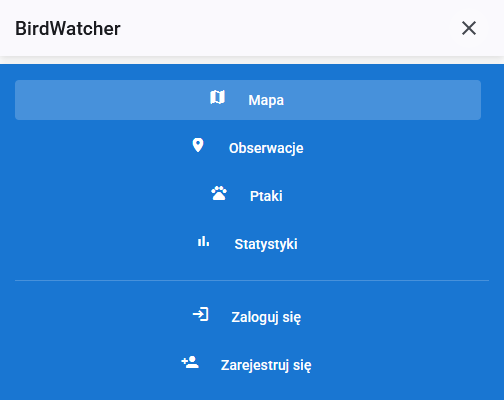
\includegraphics[width=0.6\textwidth]{/chapter4/navbar2.png}
	\caption{Pasek nawigacyjny w trybie rozwijanym}
	\label{fig:navbar2}
\end{figure}

\subsubsection{Strona główna}
Strona główna zawiera interaktywną mapę wyświetlająca obserwację zaznaczone pinezkami z podziałem na tygodnie w roku.

\begin{figure}[!htb]
	\centering
	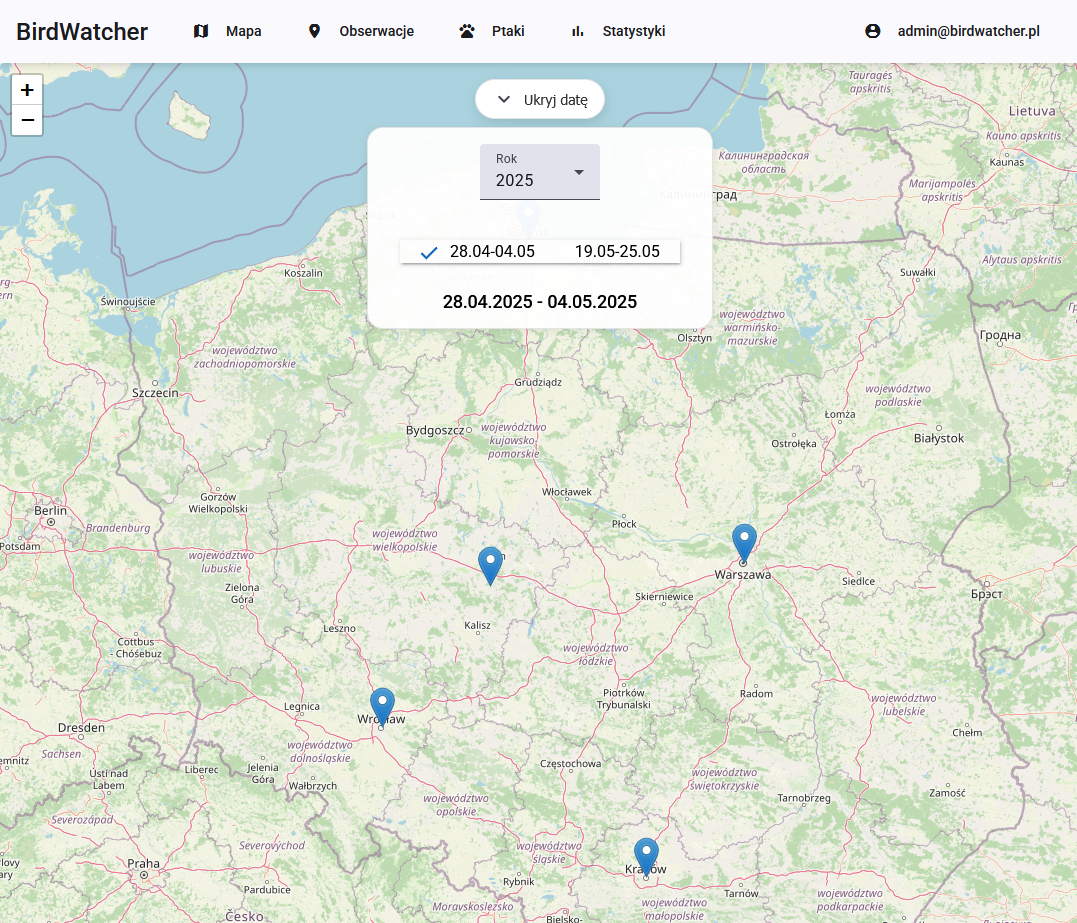
\includegraphics[width=0.6\textwidth]{/chapter4/mainpage1.png}
	\caption{Strona główna z mapą interaktywną}
	\label{fig:mainpage1}
\end{figure}

\subsubsection{Komponenty ptaków}
Zaimplementowane zostały następujące komponenty ptaków:
\begin{itemize}
	\item Lista ptaków
	\item Formularz dodawania oraz edycji ptaków
	\item Strona szczegółów ptaka
\end{itemize}

\begin{figure}[!htb]
	\centering
	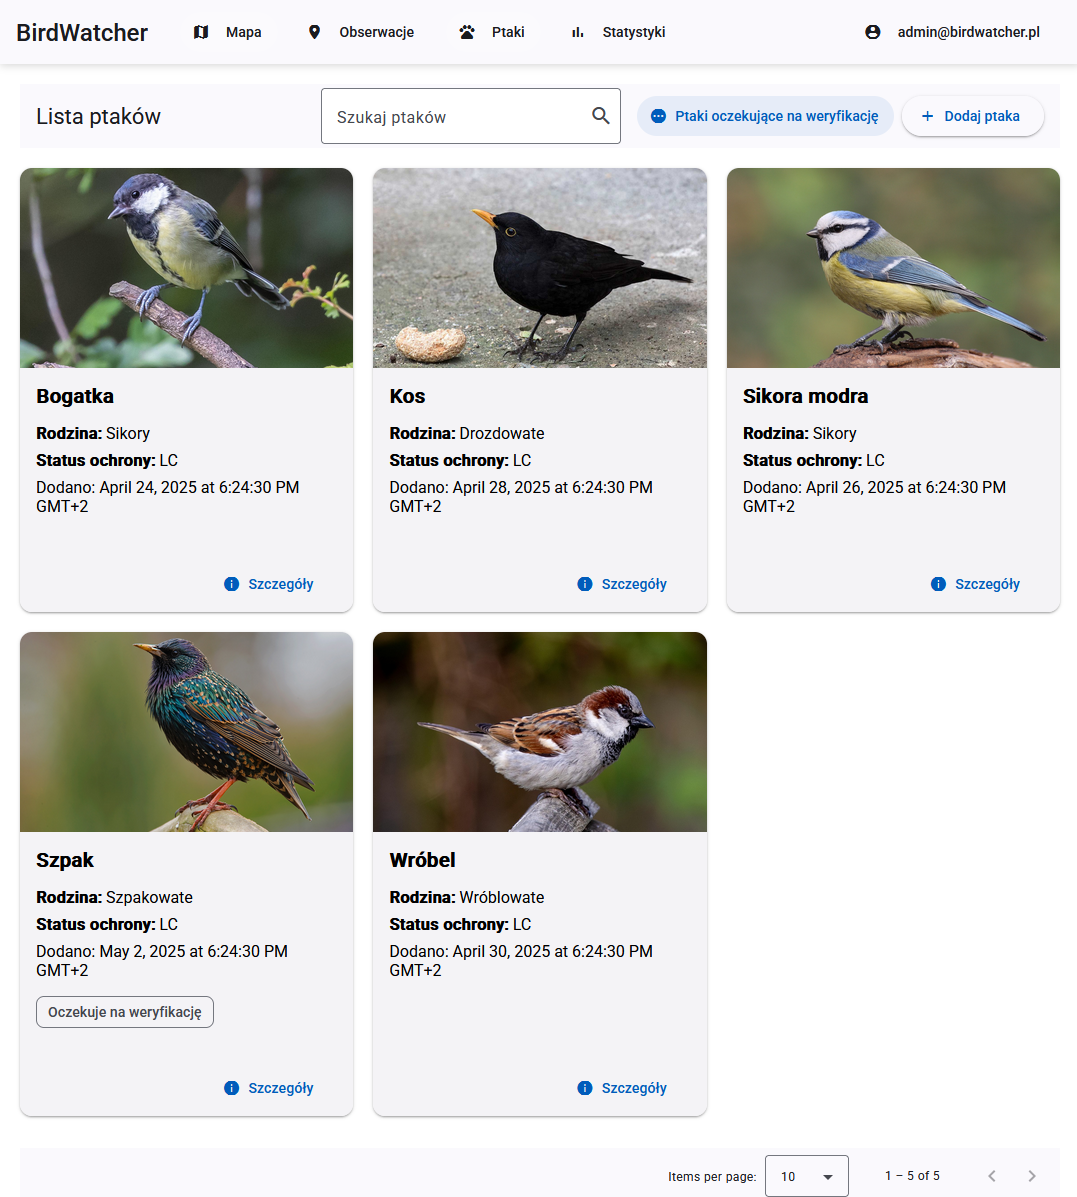
\includegraphics[width=0.6\textwidth]{/chapter4/ptaki1.png}
	\caption{Strona listy ptaków}
	\label{fig:ptaki1}
\end{figure}

\begin{figure}[!htb]
	\centering
	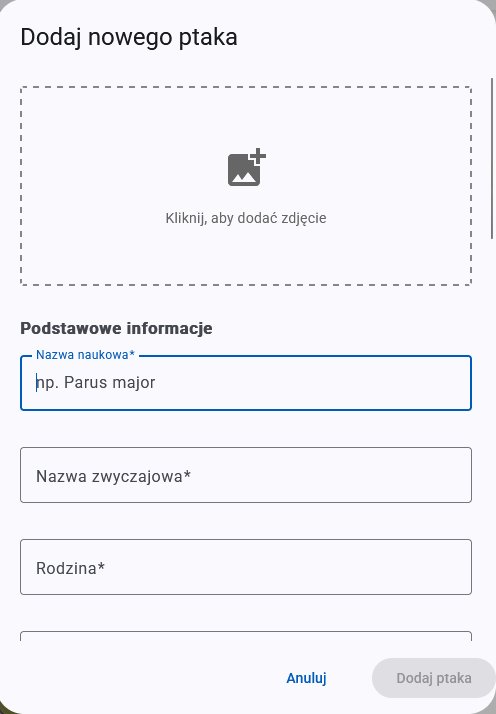
\includegraphics[width=0.4\textwidth]{/chapter4/ptaki2.png}
	\caption{Formularz dodawania/edycji ptaka}
	\label{fig:ptaki2}
\end{figure}

\begin{figure}[!htb]
	\centering
	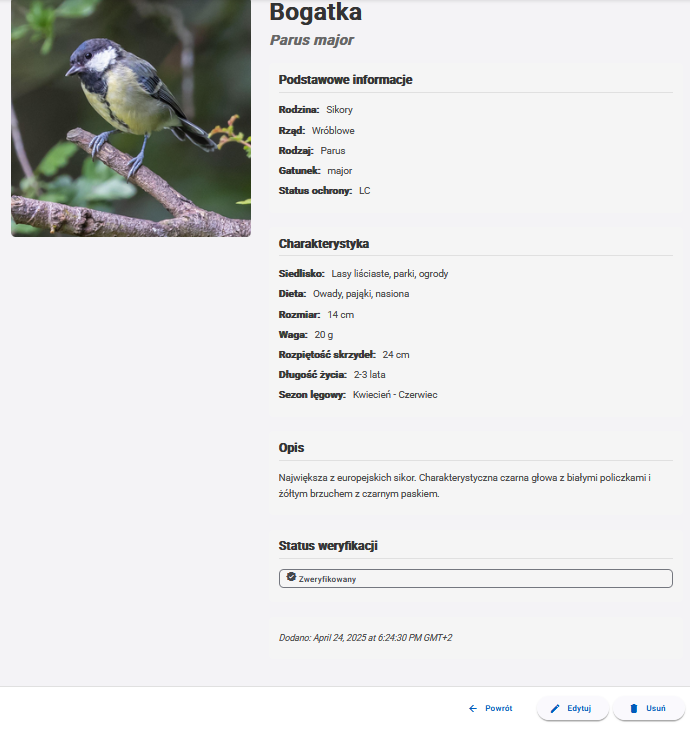
\includegraphics[width=0.6\textwidth]{/chapter4/ptaki3.png}
	\caption{Strona szczegółów ptaka}
	\label{fig:ptaki3}
\end{figure}

\subsubsection{Komponenty obserwacji}
Zaimplementowane zostały następujące komponenty związane z obserwacjami:
\begin{itemize}
	\item Lista obserwacji ptaków
	\item Formularz dodawania oraz edycji obserwacji
	\item Strona szczegółów obserwacji wraz z galerią obrazów
\end{itemize}

\begin{figure}[!hb]
	\centering
	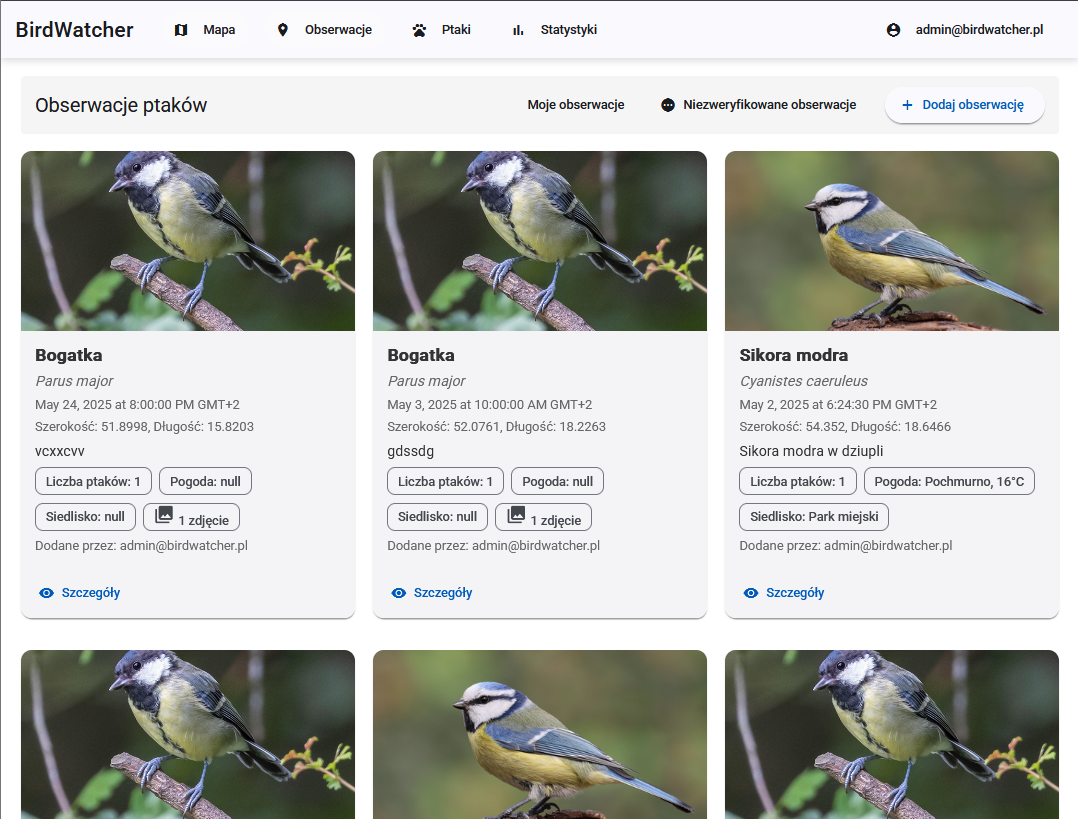
\includegraphics[width=0.6\textwidth]{/chapter4/obserwacje1.png}
	\caption{Strona listy obserwacji}
	\label{fig:obserwacje1}
\end{figure}

\begin{figure}[!hb]
	\centering
	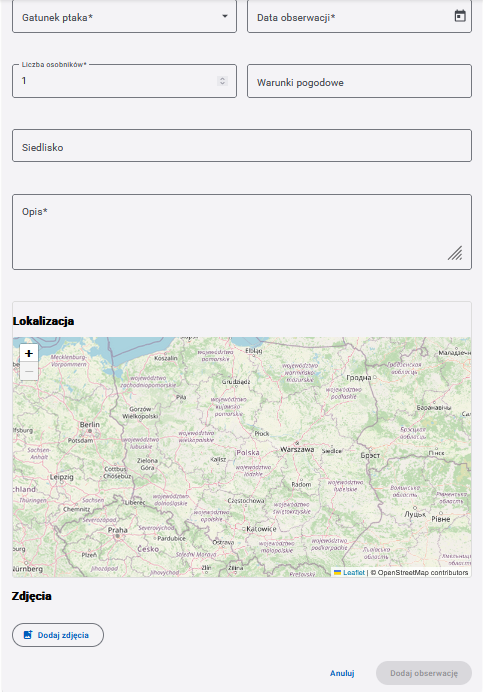
\includegraphics[width=0.4\textwidth]{/chapter4/obserwacje2.png}
	\caption{Formularz dodawania/edycji obserwacji}
	\label{fig:obserwacje2}
\end{figure}

\begin{figure}[!htb]
	\centering
	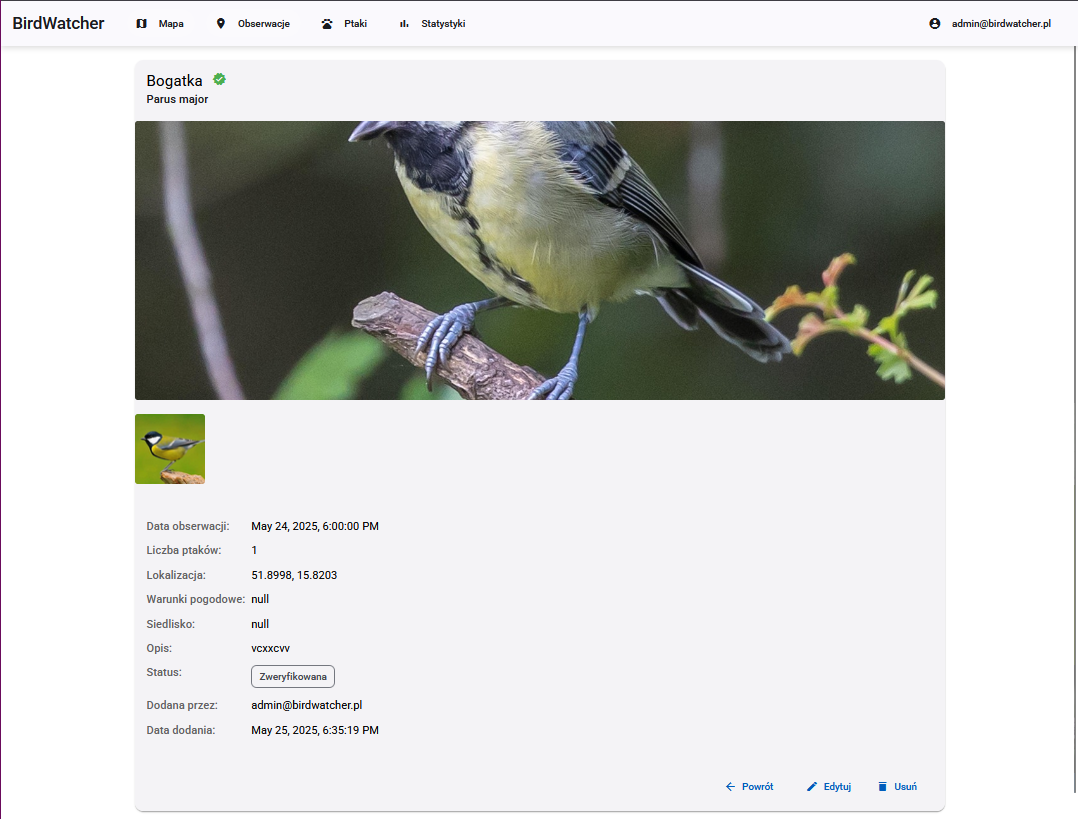
\includegraphics[width=0.6\textwidth]{/chapter4/obserwacje3.png}
	\caption{Strona szczegółów obserwacji}
	\label{fig:obserwacje3}
\end{figure}

\subsubsection{Komponenty użytkownika}
Zaimplementowane zostały następujące komponenty związane z użytkownikami:
\begin{itemize}
	\item Formularz logowania
	\item Formularz rejestracji
	\item Formularz zmiany danych użytkownika
\end{itemize}

\begin{figure}[!htb]
	\centering
	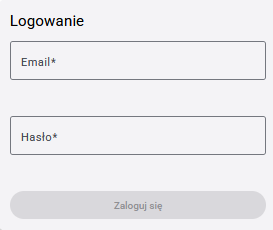
\includegraphics[width=0.6\textwidth]{/chapter4/logowanie.png}
	\caption{Formularz logowania}
	\label{figlogowanie}
\end{figure}

\begin{figure}[!htb]
	\centering
	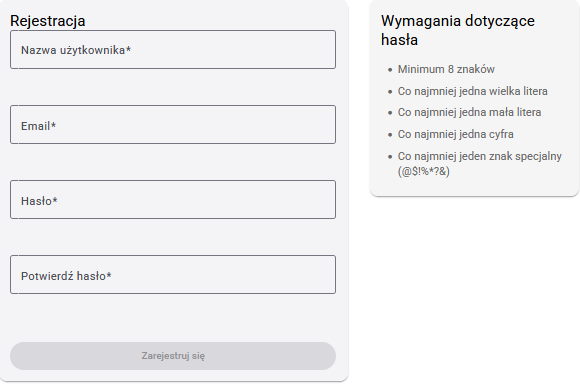
\includegraphics[width=0.6\textwidth]{/chapter4/rejestracja.png}
	\caption{Formularz rejestracji}
	\label{fig:rejestracja}
\end{figure}

\begin{figure}[!htb]
	\centering
	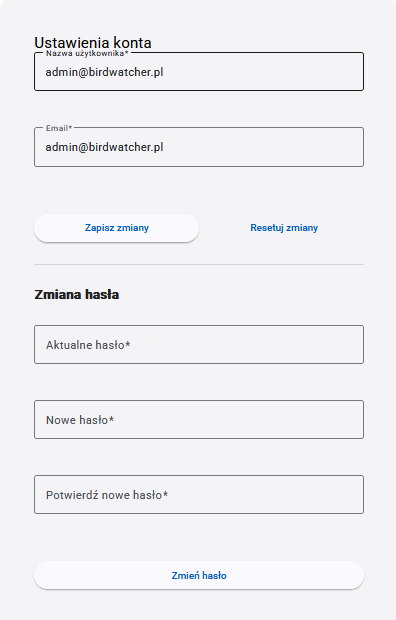
\includegraphics[width=0.6\textwidth]{/chapter4/konto.png}
	\caption{Formularz konta użytkownika}
	\label{fig:konto}
\end{figure}

\subsection{Podsumowanie implementacji frontendu}
\index{Podsumowanie implementacji frontendu}

Aplikacja frontendowa wykonana w technologii Angular została stworzona zgodnie z przyjętymi koncepcjami Angular oraz praktykując najlepsze techniki programowania obiektowego i wzorcami projektowymi. Wykorzystanie komponentów Material znacznie przyśpieszyło pracę nad systemem oraz zapewniło spójny wygląd aplikacji. Strona jest responsywna, dostosowuje się do różnych rozmiarów ekranów i ma przejrzysty interfejs. Dzięki zastosowaniu REST API, gdzie większość wymagających operacji na danyc odbywa się na backendzie i wykorzystaniu techniki paginacji aplikacja działa szybko i nie wymaga dużych zasobów mocy do działania po stronie klienta.

\FloatBarrier

\section{Implementacja backendu}
\index{Implementacja backendu}

\subsection{Architektura aplikacji backendowej}
\index{Architektura aplikacji backendowej}
Backend został stworzony przy użyciu frameworka ASP.NET Core 8.0. W aplikacji wykorzystane zostały wzorce projektowe Repository Pattern oraz Dependency Injection. REST Api zostało zaprojektowane zgodnie ze standardami co zapewnia spójny interfejs komunikacji z frontendem. Podejście projektowania bazy danych opiera się na Code First - najpierw tworzy się modele danych w kodzie a następnie na ich podstawię tworzone są migrację bazy danych zawierające odpowiednie polecenia SQL do tworzenia struktury.

\subsection{Konfiguracja aplikacji}
\index{Konfiguracja aplikacji}

Główna aplikacja znajduje się w pliku Program.cs, w którym zostały skonfigurowane niezbędne komponenty dotyczące kontrolerów API, serwisów, bazy danych, bezpieczeństwa i autoryzacji.

\begin{lstlisting}[style=csharp, caption={Fragment pliku Program.cs}]
var builder = WebApplication.CreateBuilder(args);
[...]
// Add services to the container.
builder.Services.AddControllers();
builder.Services.AddEndpointsApiExplorer();
builder.Services.AddSwaggerGen();
// Add DbContext
builder.Services.AddDbContext<ApplicationDbContext>(
	options =>options.UseSqlite(builder.Configuration
		.GetConnectionString("DefaultConnection")));
// Add Identity
builder.Services.AddIdentity<ApplicationUser, IdentityRole>(options =>
{
	// Password settings[...]
	// Lockout settings[...]
	// User settings[...]
})
.AddEntityFrameworkStores<ApplicationDbContext>()
.AddDefaultTokenProviders();
// Add Authorization Policies
builder.Services.AddAuthorization(options =>
{
	options.AddPolicy("RequireAdminRole", policy =>
	policy.RequireRole(AuthorizationConstants.AdminRole));
	options.AddPolicy("RequireUserRole", policy =>
	policy.RequireRole(AuthorizationConstants.UserRole));
});
// Add CORS
builder.Services.AddCors(options => [...]
// Add Authentication
var jwtKey = builder.Configuration["Jwt:Key"];[...]
builder.Services.AddAuthentication(options =>[...]
.AddJwtBearer(options =>[...]
// Add Services
builder.Services.AddScoped<IAuthService, AuthService>();
builder.Services.AddScoped<IBirdService, BirdService>();
builder.Services.AddScoped<IBirdObservationService, BirdObservationService>();
var app = builder.Build();
// Automatyczne tworzenie bazy danych i inicjalizacja danych
[...]
// Configure the HTTP request pipeline.
if (app.Environment.IsDevelopment())
{
	app.UseSwagger();
	app.UseSwaggerUI();
}
[...]
app.UseHttpsRedirection();
app.UseStaticFiles(); // Dodaj obsługę statycznych plików
app.UseCors("AllowAngularDevServer");
app.UseAuthentication();
app.UseAuthorization();
app.MapControllers();
app.Run();
\end{lstlisting}

\subsection{Model danych}
\index{Model danych}

\subsubsection{Kontekst bazy danych}
System wykorzystuje ORM Entity Framework Core z bazą danych SQLite. Kontekst bazy danych \texttt{ApplicationDbContext} dziedziczy po \texttt{IdentityDbContext<ApplicationUser>} co umożliwia integrację z systemem autoryzacji ASP.NET Core Identity.

\begin{lstlisting}[style=csharp, caption={Implementacja ApplicationDbContext}]
namespace BackendService.Data
{
	public class ApplicationDbContext : IdentityDbContext<ApplicationUser>
	{
		public ApplicationDbContext(DbContextOptions
		<ApplicationDbContext> options)
		: base(options)
		{}
		
		public DbSet<Bird> Birds { get; set; }
		public DbSet<BirdObservation> BirdObservations { get; set; }
		
		protected override void OnModelCreating(ModelBuilder modelBuilder)
		{
			base.OnModelCreating(modelBuilder);
			
			modelBuilder.Entity<Bird>()
			.HasOne<ApplicationUser>()
			.WithMany()
			.HasForeignKey(b => b.UserId)
			.OnDelete(DeleteBehavior.Restrict);
			
			modelBuilder.Entity<BirdObservation>()
			.HasOne(b => b.Bird)
			.WithMany(b => b.Observations)
			.HasForeignKey(b => b.BirdId)
			.OnDelete(DeleteBehavior.Cascade);
		}
	}
}
\end{lstlisting}

\subsubsection{Modele domenowe}
Aplikacja zawiera kilka klas zawierających modele domenowe:
\begin{itemize}
	\item \texttt{ApplicationUser} - rozszerzony model użytkownika z ASP.NET Core Identity
	\item \texttt{Bird} - model danych ptaka
	\item \texttt{BirdObservation} - model danych obserwacji
\end{itemize}

\begin{lstlisting}[style=csharp, caption={Implementacja ApplicationUser}]
public class ApplicationUser : IdentityUser
{
	public string? RefreshToken { get; set; }
	public DateTime? RefreshTokenExpiryTime { get; set; }
	public DateTime CreatedAt { get; set; } = DateTime.UtcNow;
	public ICollection<Bird> Birds { get; set; } = new List<Bird>();
	public ICollection<BirdObservation> BirdObservations { get; set; } = new List<BirdObservation>();
}
\end{lstlisting}

\begin{lstlisting}[style=csharp, caption={Fragment implementacji Bird}]
public class Bird
{
	public int Id { get; set; }
	
	[Required]
	public string CommonName { get; set; } = string.Empty;
	
	[Required]
	public string ScientificName { get; set; } = string.Empty;
	
	[Required]
	public string Family { get; set; } = string.Empty;
	
	public string? Order { get; set; }
	public string? Genus { get; set; }
	public string? Species { get; set; }
...
\end{lstlisting}

\begin{lstlisting}[style=csharp, caption={Fragment implementacji BirdObservation}]
public class BirdObservation
{
	public int Id { get; set; }
	
	[Required]
	public int BirdId { get; set; }
	public Bird Bird { get; set; } = null!;
	
	[Required]
	public string UserId { get; set; } = string.Empty;
	public ApplicationUser User { get; set; } = null!;
	
	[Required]
	public double Latitude { get; set; }
...
\end{lstlisting}

\subsection{Kontrolery API}
\index{Kontrolery API}

Architektura kontrolerów została zaprojektowana zgodnie z wzorcem REST API - każdy kontroler odpowiada za konkretną część domeny biznesowej. Wszystkie kontrolery dziedziczą po \texttt{ControllerBase} i są oznaczone atrybutami \texttt{[ApiController]} oraz \texttt{[Route("api/[controller]")]} co w ASP.NET Core automatycznie generuje ścieżki API na podstawie nazw kontrolerów oraz metod.

\begin{lstlisting}[style=csharp, caption={Fragment implementacji BirdsObervationsController}]
namespace BackendService.Controllers
{
	[ApiController]
	[Route("api/[controller]")]
	public class BirdObservationsController : ControllerBase
	{
		private readonly IBirdObservationService _observationService;
		
		public BirdObservationsController(IBirdObservationService observationService)
		{
			_observationService = observationService;
		}
		
		[HttpGet]
		public async Task<ActionResult<PaginatedResponse<
			BirdObservationDto>>> GetObservations([FromQuery] PaginationParams paginationParams)
		{
			var observations = await _observationService.GetAllObservationsAsync(
				paginationParams);
			return Ok(observations);
		}
		
		[HttpGet("user")]
		[Authorize]
		public async Task<ActionResult<PaginatedResponse<
			BirdObservationDto>>> GetUserObservations([FromQuery] PaginationParams paginationParams)
		{
			var userId = User.FindFirst(ClaimTypes.NameIdentifier)?.Value;
			if (string.IsNullOrEmpty(userId))
			{
				return Unauthorized();
			}
			
			var observations = await _observationService.GetUserObservationsAsync(
				userId, paginationParams);
			return Ok(observations);
		}
...
\end{lstlisting}

\subsection{Warstwa serwisów}
\index{Warstwa serwisów}
System wykorzystuje wzorzec \texttt{Dependency Injection} do zarządzania zależnościami. Serwisy są rejestrowane w \texttt{kontenerze DI} w pliku \texttt{Program.cs}

\begin{lstlisting}[style=csharp, caption={Fragment Program.cs z rejestrowaniem serwisów}]
builder.Services.AddScoped<IAuthService, AuthService>();
builder.Services.AddScoped<IBirdService, BirdService>();
builder.Services.AddScoped<IBirdObservationService, BirdObservationService>();
\end{lstlisting}

\subsection{Obsługa plików}
\index{Obsługa plików}
Aplikacja obsługuje przesyłanie i zapisywanie na backendzie plików graficznych. Pliki te są elementami ptaków oraz obserwacji. Pliki zapisywane są w katalogu \texttt{wwwroot/uploads} z unikalnymi nazwami generowanymi na podstawię \texttt{GUID} i są widoczne z poziomu aplikacji frontendowej.

\begin{lstlisting}[style=csharp, caption={Fragment implementacji zapisu plików}]
private async Task<string> SaveImageAsync(IFormFile image)
{
	var uniqueFileName = $"{Guid.NewGuid()}_{image.FileName}";
	var filePath = Path.Combine(_uploadFolder, uniqueFileName);
	
	using (var fileStream = new FileStream(filePath, FileMode.Create))
	{
		await image.CopyToAsync(fileStream);
	}
	
	return $"/uploads/birds/{uniqueFileName}";
}
\end{lstlisting}

\subsection{Walidacja danych}
\index{Walidacja danych}
Modele danych wykorzystują \texttt{[Data Adnnotations]} do walidacji prawidłowości danych po stronie serwisów.

\begin{lstlisting}[style=csharp, caption={Przykład stosowania adnotacji w modelu DTO}]
public class CreateBirdDto
{
	[Required]
	public string CommonName { get; set; } = string.Empty;
	
	[Required]
	public string ScientificName { get; set; } = string.Empty;
	
	[Required]
	public string Family { get; set; } = string.Empty;
	
	[Required]
	public string ConservationStatus { get; set; } = string.Empty;
	
	[Required]
	[MaxLength(1000)]
	public string Description { get; set; } = string.Empty;
	
	public IFormFile? Image { get; set; }
}
\end{lstlisting}

\subsection{Paginacja}
\index{Paginacja}
Aplikacja wykorzystuje dzielenie danych na mniejsze zbiory podczas prezentowania list. Zapewnia to wysoką wydajność aplikacji frontendowej oraz szybkie przesyłanie danych w mniejszych porcjach w przypadku dużych zbiorów.

\begin{lstlisting}[style=csharp, caption={Implementacja paginacji po stronie backendu}]
public class PaginationParams
{
	private const int MaxPageSize = 50;
	private int _pageSize = 10;
	
	public int PageNumber { get; set; } = 1;
	public int PageSize
	{
		get => _pageSize;
		set => _pageSize = value > MaxPageSize ? MaxPageSize : value;
	}
}

public class PaginatedResponse<T>
{
	public IEnumerable<T> Items { get; set; } = new List<T>();
	public int TotalCount { get; set; }
	public int PageNumber { get; set; }
	public int PageSize { get; set; }
	public int TotalPages { get; set; }
	public bool HasPreviousPage { get; set; }
	public bool HasNextPage { get; set; }
}
\end{lstlisting}

\subsection{Obsługa błędów}
\index{Obsługa błędów}
System implementuje globalną obsługę wyjątków poprzez wykorzystanie \texttt{middleware} oraz zwracanie odpowiednich kodów \texttt{HTTP} zgodnie z obowiązującymi standardami.

\begin{lstlisting}[style=csharp, caption={Przykład obsługi błędów w kontrolerze}]
[HttpPut("{id}")]
[Authorize(Roles = AuthorizationConstants.AdminRole)]
public async Task<IActionResult> UpdateBird(int id, [FromForm] UpdateBirdDto birdDto)
{
	try
	{
		await _birdService.UpdateBirdAsync(id, birdDto);
		return NoContent();
	}
	catch (KeyNotFoundException)
	{
		return NotFound();
	}
	catch (UnauthorizedAccessException)
	{
		return Forbid();
	}
}
\end{lstlisting}

\subsection{Konfiguracja CORS}
CORS zostały odpowiednio skonfigurowane w pliku \texttt{Program.cs} aby umożliwić obsługę żądań aplikacji frontendowej Angular.

\begin{lstlisting}[style=csharp, caption={Konfiguracja CORS}]
builder.Services.AddCors(options =>
{
	options.AddPolicy("AllowAngularDevServer",
	builder => builder
	.WithOrigins("http://localhost:4200", "https://localhost:4200")
	.AllowAnyMethod()
	.AllowAnyHeader()
	.WithExposedHeaders("Token-Expired")
	.AllowCredentials());
});
\end{lstlisting}

\subsection{Interfejs Swagger}
\index{Interfejs Swagger}
Lista \texttt{endpointów} oraz struktur wykorzystywanych w REST API jest przedstawiona w interfejsie Swagger zawartym w dodatku \ref{chapter:dodatek_A}. Dzięki interfejsowi Swagger z łatwością testuje się implementowane API oraz ułatwia on implementacje komunikacji po stronie frontendu.

\subsection{Podsumowanie implementacji backendu}
\index{Podsumowanie implementacji backendu}
Część backendowa aplikacji została zaprojektowana zgodnie z obowiązującymi najlepszymi praktykami programowania, wzorcami projektowymi oraz zaleceniami Microsoftu. Stworzony system jest modularny, łatwy w rozwoju, wydajny i bezpieczny dzięki wykorzystaniu \texttt{ASP.NET Core} w połączeniu z \texttt{Entity Framework Core}. Architektura REST API zapewnia efektywną komunikację, a implementacja paginacji wydajność ładowania danych i oszczędność zasobów.

\section{Implementacja bazy danych}
\index{Implementacja bazy danych}
Baza danych w systemie została zaimplementowana z użyciem \texttt{SQLite3} oraz \texttt{Entity Framework Core} wykorzystując podejście \texttt{code first}.

\subsection{Konfiguracja połączenia z bazą danych}
\index{Konfiguracja połączenia z bazą danych}
Połączenie z bazą danych zostało skonfigurowane w pliku \texttt{appsettings.json}

\begin{lstlisting}[style=csharp, caption={Konfiguracja bazy w appsettings.json}]
{
	"ConnectionStrings": {
		"DefaultConnection": "Data Source=birdwatcher.db"
	}
}
\end{lstlisting}

Plik bazy danych \texttt{birdwatcher.db} jest automatycznie tworzony przy pierwszym starcie aplikacji oraz automatycznie aktualizowany gdy powstają nowe migracje.

\subsection{Struktura bazy danych}
\index{Struktura bazy danych}

\subsubsection{Tabela AspNetUsers (Identity)}
Tabela \texttt{AspNetUsers} jest częścią systemu \texttt{ASP.NET Core Identity}, została rozszerzona o dodatkowe pola potrzebne w systemie i służy ona do przechowywania danych o użytkownikach.

\begin{lstlisting}[style=sqlstyle, caption={Struktura tabeli AspNetUsers}]
CREATE TABLE AspNetUsers (
	Id TEXT PRIMARY KEY,
	UserName TEXT,
	NormalizedUserName TEXT,
	Email TEXT,
	NormalizedEmail TEXT,
	EmailConfirmed INTEGER,
	PasswordHash TEXT,
	SecurityStamp TEXT,
	ConcurrencyStamp TEXT,
	PhoneNumber TEXT,
	PhoneNumberConfirmed INTEGER,
	TwoFactorEnabled INTEGER,
	LockoutEnd TEXT,
	LockoutEnabled INTEGER,
	AccessFailedCount INTEGER,
	RefreshToken TEXT,
	RefreshTokenExpiryTime TEXT,
	CreatedAt TEXT NOT NULL
);
\end{lstlisting}

\subsubsection{Tabela AspNetRoles (Identity)}
Tabela \texttt{AspNetRoles} przechowuje informację o rolach użytkowników.

\begin{lstlisting}[style=sqlstyle, caption={Struktura tabeli AspNetRoles}]
CREATE TABLE AspNetRoles (
	Id TEXT PRIMARY KEY,
	Name TEXT,
	NormalizedName TEXT,
	ConcurrencyStamp TEXT
);
\end{lstlisting}

\subsubsection{Tabela AspNetUserRoles (Identity)}
Tabela \texttt{AspNetUserRoles} łaczy użytkowników z rolami.

\begin{lstlisting}[style=sqlstyle, caption={Struktura tabeli AspNetRoles}]
CREATE TABLE AspNetUserRoles (
	UserId TEXT NOT NULL,
	RoleId TEXT NOT NULL,
	PRIMARY KEY (UserId, RoleId),
	FOREIGN KEY (UserId) REFERENCES AspNetUsers(Id) ON DELETE CASCADE,
	FOREIGN KEY (RoleId) REFERENCES AspNetRoles(Id) ON DELETE CASCADE
);
\end{lstlisting}

\subsubsection{Tabela Birds}
Tabela \texttt{Birds} przechowuje informację o ptakach.

\begin{lstlisting}[style=sqlstyle, caption={Struktura tabeli AspNetRoles}]
CREATE TABLE Birds (
	Id INTEGER PRIMARY KEY AUTOINCREMENT,
	CommonName TEXT NOT NULL,
	ScientificName TEXT NOT NULL,
	Family TEXT NOT NULL,
	Order TEXT,
	Genus TEXT,
	Species TEXT,
	ConservationStatus TEXT NOT NULL,
	Description TEXT NOT NULL,
	Habitat TEXT,
	Diet TEXT,
	Size TEXT,
	Weight REAL,
	Wingspan REAL,
	Lifespan TEXT,
	BreedingSeason TEXT,
	ImageUrl TEXT,
	IsVerified INTEGER NOT NULL DEFAULT 0,
	UserId TEXT NOT NULL,
	CreatedAt TEXT NOT NULL,
	FOREIGN KEY (UserId) REFERENCES AspNetUsers(Id) ON DELETE RESTRICT
);
\end{lstlisting}

\subsubsection{Tabela BirdObervations}
Tabela \texttt{BirdObersvations} przechowuje informację o obserwacjach ptaków.

\begin{lstlisting}[style=sqlstyle, caption={Struktura tabeli AspNetRoles}]
CREATE TABLE BirdObservations (
	Id INTEGER PRIMARY KEY AUTOINCREMENT,
	BirdId INTEGER NOT NULL,
	UserId TEXT NOT NULL,
	Latitude REAL NOT NULL,
	Longitude REAL NOT NULL,
	ObservationDate TEXT NOT NULL,
	Description TEXT,
	NumberOfBirds INTEGER,
	WeatherConditions TEXT,
	Habitat TEXT,
	IsVerified INTEGER NOT NULL DEFAULT 0,
	CreatedAt TEXT NOT NULL,
	UpdatedAt TEXT NOT NULL,
	ImageUrls TEXT NOT NULL DEFAULT '[]',
	FOREIGN KEY (BirdId) REFERENCES Birds(Id) ON DELETE CASCADE,
	FOREIGN KEY (UserId) REFERENCES AspNetUsers(Id) ON DELETE CASCADE
);
\end{lstlisting}

\newpage

\subsection{Relacje}
\index{Relacje}

\subsubsection{Diagram relacji}

\begin{figure}[!htb]
	\centering
	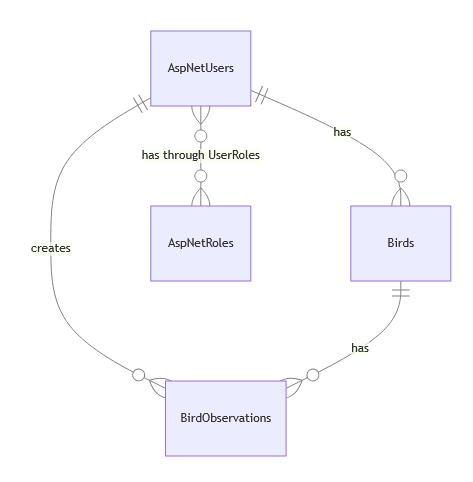
\includegraphics[width=0.6\textwidth]{/chapter4/diagramrelacji.png}
	\caption{Uproszczony diagram relacji bazy danych}
	\label{fig:diagramrelacji}
\end{figure}

\subsubsection{Konfiguracja relacji w Entity Framework Core}

\begin{lstlisting}[style=csharp, caption={Konfiguracja relacji w Entity Framework Core}]
protected override void OnModelCreating(ModelBuilder modelBuilder)
{
	base.OnModelCreating(modelBuilder);
	
	modelBuilder.Entity<Bird>()
	.HasOne<ApplicationUser>()
	.WithMany()
	.HasForeignKey(b => b.UserId)
	.OnDelete(DeleteBehavior.Restrict);
	
	modelBuilder.Entity<BirdObservation>()
	.HasOne(b => b.Bird)
	.WithMany(b => b.Observations)
	.HasForeignKey(b => b.BirdId)
	.OnDelete(DeleteBehavior.Cascade);
}
\end{lstlisting}

\subsection{Indeksy bazy danych}
\index{Indeksy bazy danych}
W bazie danych zostały utworzone następujące indeksy aby poprawić wydajność wyszukiwania.

\begin{lstlisting}[style=sqlstyle, caption={Indeksy bazy danych}]
-- Indeksy dla tabeli Birds
CREATE INDEX IX_Birds_CommonName ON Birds(CommonName);
CREATE INDEX IX_Birds_ScientificName ON Birds(ScientificName);

-- Indeksy dla tabeli BirdObservations
CREATE INDEX IX_BirdObservations_BirdId ON BirdObservations(BirdId);
CREATE INDEX IX_BirdObservations_UserId ON BirdObservations(UserId);
CREATE INDEX IX_BirdObservations_ObservationDate ON BirdObservations(ObservationDate);
CREATE INDEX IX_BirdObservations_Latitude_Longitude ON BirdObservations(Latitude, Longitude);

-- Indeksy dla tabeli AspNetUsers (Identity)
CREATE INDEX IX_AspNetUsers_Email ON AspNetUsers(Email);
CREATE INDEX IX_AspNetUsers_UserName ON AspNetUsers(UserName);
\end{lstlisting}

\subsection{Migracje}
\index{Migracje}
W aplikacji wykorzystywany jest \texttt{Code-First Migrations Entity Framework Core} do zarządzania schematem bazy danych.
Historia migracji jest przechowywana w osobnych plikach nazwanych opisowo np.:
\begin{enumerate}
	\item InitalCreate
	\item AddBirdsAndObserwations
	\item AddRefreshToken
	\item ...
\end{enumerate}


Przykład jak wygląda migracja:

\begin{lstlisting}[style=csharp, caption={Przykład migracji bazy danych}]
public partial class AddObservationImages : Migration
{
	protected override void Up(MigrationBuilder migrationBuilder)
	{
		migrationBuilder.AddColumn<string>(
		name: "ImageUrls",
		table: "BirdObservations",
		type: "TEXT",
		nullable: false,
		defaultValue: "[]");
	}
	
	protected override void Down(MigrationBuilder migrationBuilder)
	{
		migrationBuilder.DropColumn(
		name: "ImageUrls",
		table: "BirdObservations");
	}
}
\end{lstlisting}

\subsection{Backup i odzyskiwanie}
\index{Backup i odzyskiwanie}
Ponieważ SQLite przechowuje bazę danych jako jeden plik na dysku, backup sprowadza się do skopiowania pliku \texttt{birdwatcher.db}

\begin{lstlisting}[language=bash, caption={Przykład skryptu kopiującego w bash}]
cp birdwatcher.db backup/birdwatcher_$(date +%Y%m%d_%H%M%S).db
\end{lstlisting}

\subsection{Automatyczne tworzenie bazy danych}
\index{Automatyczne tworzenie bazy danych}
Automatyczne tworzenie bazy danych zostało zaimplementowane w pliku \texttt{Program.cs}.

\begin{lstlisting}[style=csharp, caption={Automatyczne tworzenie bazy danych}]
using (var scope = app.Services.CreateScope())
	{
		var services = scope.ServiceProvider;
		try
		{
			var context = services.GetRequiredService
			<ApplicationDbContext>();
			context.Database.EnsureCreated();
			await SeedData.Initialize(services);
		}
		catch (Exception ex)
		{
			var logger = services.GetRequiredService<ILogger<Program>>();
			logger.LogError(ex, "Wystąpił błąd podczas tworzenia bazy danych.");
		}
	}
\end{lstlisting}

\subsection{Podsumowanie implementacji bazy danych}
\index{Podsumowanie implementacji bazy danych}
Baza danych aplikacji została zaprojektowana by być łatwo w rozwoju oraz przechowywaniu. Dzięki podejściu \texttt{code first} oraz wykorzystaniu mechanizmów migracji dodanie nowych modeli oraz modyfikacja istniejących jest szybka i łatwa w realizacji. Dodatkowo mechanizmy \texttt{ASP.NET Core Identity} dostarczają gotowe rozwiązania zarządzania użytkownikami i schemat danych.

\FloatBarrier

\section{Implementacja systemu autentyfikacji i autoryzacji}
\index{Implementacja systemu autentyfikacji i autoryzacji}
System autentykacji i autoryzacji w aplikacji składa się z kilku nowoczesnych technologii i najlepszych praktyk bezpieczeństwa. Wykorzystuje on do działania \texttt{JWT (JSON Web Tokens)} w połączeniu z tokenami odświeżającymi oraz system ról oparty na \texttt{ASP.NET Core Identity}

\subsection{Architektura systemu autentykacji}
\index{Architektura systemu autentykacji}
System składa się z paru kluczowych elementów:
\begin{itemize}
	\item \textbf{Model użytkownika} - rozszerzenie \texttt{IdentityUser} o dodatkowe pola
	\item \textbf{Serwis autentykacji} - logika biznesowa związana z autentykacją
	\item \textbf{Kontroler autentykacji} - endpointy REST API
	\item \textbf{Interceptor HTTP} - automatyczne dodawanie tokenów autoryzacji do żądań po stronie frontendu
	\item \textbf{Serwis frontendowy} - zarządzający stanem autentykacji po stronie klienta
\end{itemize}

\subsection{Konfiguracja Identity i JWT}
\index{Konfiguracja Identity i JWT}
W pliku \texttt{Program.cs} skonfigurowany został system autentykacji \texttt{Identity} poprzez wskazanie odpowiednich opcji bezpieczeństwa:

\begin{lstlisting}[style=csharp, caption={Konfiguracja bezpieczeństwa w Program.cs}]
builder.Services.AddIdentity<ApplicationUser, IdentityRole>(options =>
{
	// Ustawienia haseł
	options.Password.RequireDigit = true;
	options.Password.RequireLowercase = true;
	options.Password.RequireUppercase = true;
	options.Password.RequireNonAlphanumeric = true;
	options.Password.RequiredLength = 8;
	
	// Ustawienia blokady konta
	options.Lockout.DefaultLockoutTimeSpan = TimeSpan.FromMinutes(15);
	options.Lockout.MaxFailedAccessAttempts = 5;
	options.Lockout.AllowedForNewUsers = true;
	
	// Ustawienia użytkownika
	options.User.RequireUniqueEmail = true;
	options.SignIn.RequireConfirmedEmail = false;
})
.AddEntityFrameworkStores<ApplicationDbContext>()
.AddDefaultTokenProviders();
\end{lstlisting}

Konfiguracja JWT obejmuję walidację tokenów z odpowiednimi parametrami bezpieczeństwa:

\begin{lstlisting}[style=csharp, caption={Konfiguracja JWT w Program.cs}]
builder.Services.AddAuthentication(options =>
{
	options.DefaultAuthenticateScheme = JwtBearerDefaults.AuthenticationScheme;
	options.DefaultChallengeScheme = JwtBearerDefaults.AuthenticationScheme;
	options.DefaultScheme = JwtBearerDefaults.AuthenticationScheme;
})
.AddJwtBearer(options =>
{
	options.TokenValidationParameters = new TokenValidationParameters
	{
		ValidateIssuer = true,
		ValidateAudience = true,
		ValidateLifetime = true,
		ValidateIssuerSigningKey = true,
		ValidIssuer = builder.Configuration["Jwt:Issuer"],
		ValidAudience = builder.Configuration["Jwt:Audience"],
		IssuerSigningKey = new SymmetricSecurityKey(Encoding.UTF8.GetBytes(jwtKey))
	};
});
\end{lstlisting}

\subsection{System ról i autoryzacji}
\index{System ról i autoryzacji}
Zostały zdefiniowane dwie główne role w systemie:

\begin{lstlisting}[style=csharp, caption={Role w systemie}]
public static class AuthorizationConstants
{
	public const string AdminRole = "Admin";
	public const string UserRole = "User";
}
\end{lstlisting}

Odpowiednie polityki pozwalają na kontrolę dostępu użytkowników do zasobów:

\begin{lstlisting}[style=csharp, caption={Polityki autoryzacji}]
builder.Services.AddAuthorization(options =>
{
	options.AddPolicy("RequireAdminRole", policy =>
	policy.RequireRole(AuthorizationConstants.AdminRole));
	
	options.AddPolicy("RequireUserRole", policy =>
	policy.RequireRole(AuthorizationConstants.UserRole));
});
\end{lstlisting}

\subsection{Serwis autentykacji}
\index{Serwis autentykacji}
\texttt{AuthService} po stronie backendu implementuje wszystkie operacje związane z autentykacją.

\subsubsection{Logowanie użytkownika}
Proces logowania obejmuje:
\begin{itemize}
	\item Walidację danych
	\item Sprawdzanie blokady konta
	\item Weryfikacje hasła
	\item Generowanie tokenów dostępu i odświeżających
	\item Resetowanie licznika nieudanych prób
\end{itemize}

Kod odpowiedzialny za logowanie został zawarty w listingu \ref{lst:logowanie}


\subsubsection{Rejestracja użytkownika}
Proces rejestracji obejmuje:
\begin{itemize}
	\item Walidację danych
	\item Tworzenie nowego użytkownika
	\item Automatyczne przypisanie roli
	\item Generowanie tokenów dostępu po rejestracji
\end{itemize}

Kod odpowiedzialny za rejestracje został zawarty w listingu \ref{lst:rejestracja}

\subsection{Generowanie tokenów}
\index{Generowanie tokenów}
Tokeny dostępu generowane są z odpowiednimi parametrami o krótkim czasie ważności (15 minut):

\begin{lstlisting}[style=csharp, caption={Generowanie tokenu JWT}]
private string GenerateAccessToken(ApplicationUser user, IList<string> roles)
{
	var claims = new List<Claim>
	{
		new Claim(ClaimTypes.NameIdentifier, user.Id),
		new Claim(ClaimTypes.Name, user.UserName!),
		new Claim(ClaimTypes.Email, user.Email!)
	};
	
	foreach (var role in roles)
	{
		claims.Add(new Claim(ClaimTypes.Role, role));
	}
	
	var key = new SymmetricSecurityKey(Encoding.UTF8.GetBytes(
		_configuration["Jwt:Key"]!));
	var creds = new SigningCredentials(key, SecurityAlgorithms.HmacSha256);
	var expires = DateTime.UtcNow.AddMinutes(
		ACCESS_TOKEN_EXPIRATION_MINUTES);
	
	var token = new JwtSecurityToken(
	_configuration["Jwt:Issuer"],
	_configuration["Jwt:Audience"],
	claims,
	expires: expires,
	signingCredentials: creds
	);
	
	return new JwtSecurityTokenHandler().WriteToken(token);
}
\end{lstlisting}

Tokeny odświeżające są generowane przy użyciu kryptograficznie bezpiecznego generatora liczb losowych:

\begin{lstlisting}[style=csharp, caption={Generowanie tokenu odświeżającego}]
private string GenerateRefreshToken()
{
	var randomNumber = new byte[32];
	using var rng = RandomNumberGenerator.Create();
	rng.GetBytes(randomNumber);
	return Convert.ToBase64String(randomNumber);
}
\end{lstlisting}

\subsection{Kontroler autentykacji}
\index{Kontroler autentykacji}
\texttt{AuthController} udostępnia następujące endpointy REST API dla operacji autentykacji:
\begin{itemize}
	\item /api/auth/login
	\item /api/auth/register
	\item /api/auth/refresh-token
	\item /api/auth/logout
\end{itemize}

Implementacja kontrolera została przedstawiona w listingu \ref{lst:kontrolerautentykacji}

\subsection{Frontend - Serwis autentyfikacji}
\index{Frontend - Serwis autentyfikacji}
W aplikacji frontendowej Angular zaimplementowano \texttt{AuthService} odpowiedzialny za zarządzaniestanem autentyfikacji użytkownika.
Serwis implementuje przechowywanie tokenu, kontrole nad zalogowanym użytkownikiem, odświeżanie tokenu oraz wylogowywanie.

Implementacja serwisu została przedstawiona w listingu \ref{lst:serwisautentykacjifrontend}

\subsection{Interceptor HTTP}
\index{Interceptor HTTP}

Interceptor automatycznie dodaje tokeny do żądań wysyłanych z frontendu i obsługuje błędy autoryzacji.

\begin{lstlisting}[style=tsstyle, caption={Interceptor HTTP}]
export const authInterceptor: HttpInterceptorFn = (req, next) => {
	const router = inject(Router);
	const authService = inject(AuthService);
	const token = localStorage.getItem('accessToken');
	
	if (token) {
		const clonedReq = req.clone({
			headers: req.headers.set('Authorization', `Bearer ${token}`)
		});
		req = clonedReq;
	}
	
	return next(req).pipe(
	catchError((error: HttpErrorResponse) => {
		if (error.status === 401 && !req.url.includes('/refresh-token')) {
			return authService.refreshToken().pipe(
			switchMap(response => {
				const newReq = req.clone({
					headers: req.headers.set('Authorization', `Bearer ${response.accessToken}`)
				});
				return next(newReq);
			}),
			catchError(refreshError => {
				authService.logout().subscribe(() => {
					router.navigate(['/login'], {
						queryParams: { returnUrl: router.url }
					});
				});
				return throwError(() => refreshError);
			})
			);
		}
		
		if (error.status === 403) {
			router.navigate(['/login'], { 
				queryParams: { returnUrl: router.url }
			});
		}
		
		return throwError(() => error);
	})
	);
};
\end{lstlisting}

\subsection{Bezpieczeństwo systemu}
\index{Bezpieczeństwo systemu}

\subsection{Podsumowanie}
\index{Podsumowanie}

\section{Implementacja funkcjonalności mapy i geolokalizacji}
\index{Implementacja funkcjonalności mapy i geolokalizacji}